\documentclass[../main.tex]{subfiles}
\begin{document}
\chapter{実験}


本章では,4章で述べた手法で仮説を検証するための実験方法と
実験システムの設計について述べる.


\section{ツール構成}
本研究ではPythonを用いてツール作成を行った.
実装については大きく分けて3つに分けられる.
1つ目がコート作成,2つ目がパスへのタグ付け,3つ目がタグの呼び出しである.\\
1つのコート作成はcanvas上に水球のゴールや2m,5m,6mの位置に線を引いた.2つめのパスへのタグ付けについても座標から座標に白い線を引いた.
ここでは1番〜9番の各ポジションとシュートを打った際のjklの計12箇所を通るパスの全ての組み合わせに白い線を引いた.
例としては,1番から2番へのパスのタグとして'12p',4番から6番へのパスを'46p',6番からjの位置へのシュートを'6j'と設定した.
タグの呼び出し場面では,座標から座標に線を引くのではなく,タグを呼び出し指定のタグを黒い線に変えような実装を行った.
タグの呼び出しにすることで入力が楽になり,操作性の向上を図った.


\section{仕様}
\subsection{使用者の操作}
実験参加者は1本の退水セットの結果を出力するために以下の手順で本ツールを使用する.
これを10本行い,10本目は操作4で終了とした.
\par 操作1:退水セットの何本目について分析を行うのか,そしてそのセットがゴール・パス・シュートのどれに終わったのかを記入する.
\par 操作2:パスのルートに対応する事前にこちらで設定したタグを入力する.
\par 操作3:出力を行う
\par 操作4:出力結果のスクリーンショットを撮影する
\par 操作5:操作1の画面に戻る\\
今後は操作1〜3を操作画面,操作4.5をデスクトップ画面と呼ぶ.操作画面での数値各入力箇所はこのように配置されている.\ref{img:screen}
また,各操作における所要時間を測定するために捜査中の画面収録を行った.スクリーンショットの撮影日時の情報と合わせ,操作感の評価段階で使用する.


\begin{figure}[ht]
    \begin{center}
        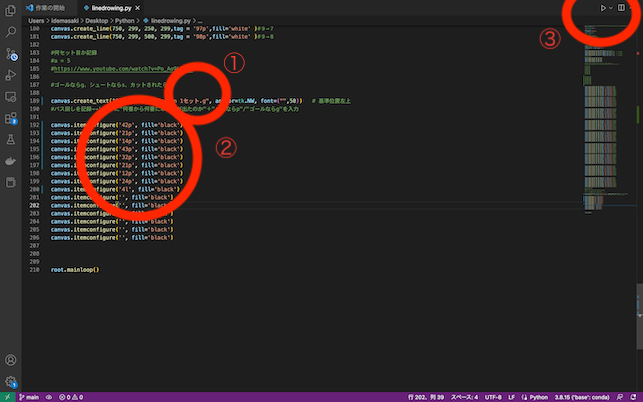
\includegraphics{img/03.png}
        \caption{本実験で使用したツールの操作画面}
        \label{img:screen}
    \end{center}
\end{figure}



\section{実験}
ここでは慶應義塾大学體育會水泳部水球部門,並びに慶應義塾高等学校水球部部員の協力の下で行った実験について述べる.

\subsection{大学生によるディフェンスへの適応実験}
ここでは大学生に対して実施した,ディフェンスに分析結果を適応する実験の詳細を述べる.\par
・実験の概要
\par 実験は大学水球の部員の協力の下,1週間かけて行った.大学生をAとBの2チームに分け選手を固定し,2度退水セットの練習を行った.1度目と2度目の退水セット間には1週間の時間を設け,
Aチームの選手には5・6番ポジションの選手を使うというコンセプトを指示した.これに対してBチームの選手がツールを用いて1週間の間にAチームの分析を行い,
コンセプトの指示内容を見抜き対策を立てられるかどうかを検証した.
\par 実験の手順は以下の通りである.
\par ①フィールドプレーヤー12名,ゴールキーパー2名をAとBの2チームに分ける.Bチームの選手には「5・6番ポジションの選手を使う」というコンセプトを指示し,
攻守それぞれ10本ずつの退水セットを行う.
\par ②Aチームの選手計7名は,筆者と1名ずつ共にツールを使用しBチームがオフェンスを行った退水セット10本の出力を行う.出力が10本終了後に操作性についての記述式アンケートを行う.
\par ③Aチームの選手には,正しい分析結果の出力結果10本分並びに分析項目が掲載された,Excelファイル{/Microsoft社提供/}を送付し,BチームのOFについて分析を行ってもらう.
\par ④分析結果を筆者が集計し,2度目の退水セットの直前に集計した分析結果を選手にフィードバックを行う.
\par ⑤1度目と同じく2度目の退水セットを攻守10本ずつ実施する.
\par ⑥退水セット終了後,1度目と2度目で比較してどのような心理的変化があったのか,アンケートを行う



\leavevmode\\
Aチームの選手が行う分析内容は以下の4つになる.
\par ①コンセプト予想
\par ②分析結果から分かること
\par ③分析結果から分からないこと
\par ④相手のコンセプトは何か


\leavevmode\\
2回目の退水セットを行った後に実施したアンケート項目は以下の4つになる.
\par ①分析後、自分達のDFに変化を感じたか:Yes・No形式
\par ②どのような変化がありましたか:記述式
\par ③DFの改善にこの分析は使えそうか::Yes・No形式




\subsection{高校生によるオフェンスへの適応実験}
ここでは高校生に対して実施した,オフェンスに分析結果を適応する実験の詳細を述べる.\par
・実験の概要
\par 実験は高校水球の部員の下,1週間かけて行った.高校生をCとDの2チームに分け選手を固定し,2度退水セットの練習を行った.1度目と2度目の退水セット間には1週間の時間を設け,1週間の間にCの選手は
ツールを用いて自分達のチームのオフェンスを分析してもらった.CとDの選手はこの分析以外には全く同じメニューを行って練習しており,同じコンセプトで退水セットを行っている.
ツールによる分析が練習内容の理解を促すのかを検証した.
\par 実験の手順は以下の通りである.
\par ①フィールドプレーヤー12名,ゴールキーパー2名をCとDの2チームに分けて退水セットを実施した.
なお本実験では,CチームDチーム共に同じコンセプトを持ってオフェンスを行った.
\par ②Cチームの選手は,2日間に渡り筆者と共に分析ツールを使用し,出力を行った.出力が10本終了後に操作性についてのアンケートを行った.
\par ③Cチームの選手には,正しい分析結果の出力結果10本分並びに分析項目が掲載された,Excelファイル{/Microsoft社提供/}を送付し,CチームのOFについて分析を行ってもらう.
\par ④分析結果を筆者が集計し,2度目の退水セットの直前に集計した分析結果を選手にフィードバックを行う.
\par ⑤1度目と同じく2度目の退水セットを攻守10本ずつ実施する.
\par ⑥退水セット終了後,1度目と2度目で比較してどのような心理的変化があったのかアンケートを行う


\leavevmode\\
Cチームの選手が行う分析内容は以下の4つになる.
\par ①決め事の中で出来たこと:記述式
\par ②分析シートを見て振り返り:記述式
\par ③改善点:記述式
\par ④ここからは不明瞭な部分:記述式


\leavevmode\\
2回目の退水セットを行ったのち,分析を行ったCチームの選手に以下の項目でアンケートを実施した。
\par ①分析後,1度目の退水セットを比較して2回目ではOFにおける変化を感じたか:Yes・No形式
\par ②どのような変化がありましたか:記述式
\par ③日々の練習でこの分析によるフィードバックは有効そうか:Yes・No形式
\par ④退水以外でどのような場面で分析が使えそうか:記述式



\end{document}